\chapter{The Tradeoff between Evolvability and Efficiency in the Evolution of Cooperation}
\label{chapter:C2_article1}

\setcounter{secnumdepth}{0}
\setcounter{minitocdepth}{1}
\minitoc[n] % minitoc without title

This Chapter is centered on the evolution of coordination behaviours in a task of collective foraging. It is organized as a published paper in an international conference:

\begin{quote}
  \fullcite{Bernard2015}
\end{quote}


We are interested in the subject of evolving cooperation among a population of heterogeneous robots. In particular, we aim at comparing an homogeneous approach (i.e. a clonal approach) and an heterogeneous approach. As we previously discussed in Chapter~\ref{chapter:design}, the classical approach to designing MRS in evolutionary robotics is to use a team of homogeneous robots. This is indeed the easiest way to ensure the evolution of cooperation because the fitness of the individuals is the same as that of the group. However, this means that we often focus only on the \emph{evolvability} of the cooperative solution, i.e. the probability to evolve cooperative individuals~\footnote{It is important to note that the term "evolvability" has a strong connotation in the field of evolutionary robotics and may correspond to various definitions. In particular, one such definition is that it conveys the capacity for an individual to adapt to environmental change~\parencite{Wagner1996}. This is a rising topic in artificial evolution~\parencite{Banzhaf2006, Lehman2013, Doncieux2015a, Taylor2016} and as such we do not want to create confusion with our use of the term here. In this Chapter, evolvability strickly refers to the capacity to evolve a particular trait (in our case, cooperation).}. However groups of heterogeneous robots may achieve greater \emph{efficiency} (in terms of fitness performance) when coordination is required. Because individuals can adopt distinct behaviours, they could evolve more diverse coordination strategies. Yet heterogeneity may hinder the evolution of cooperation in an environment where it is possible for robots to act in a selfish manner. We thus want to compare both these approaches in such an environment on these two criteria: evolvability and efficiency.

To that end, we designed a simple collective foraging task inspired by the stag hunt. More precisely, two individuals are placed in an arena where they can forage two different types of targets: green and purple. Green targets reward the same whether they are collected alone or cooperatively. In comparison, purple targets need to be collected in a cooperative fashion but reward more than the green ones. Given this setting, we are interested in the evolution of cooperative behaviours, i.e. individuals foraging the purple targets cooperatively. We study three different approaches w.r.t. team composition:

\begin{itemize}
  \item{A control setup, where both individuals come from the same population but are genetically different.}
  \item{A clonal setup, where the two individuals are clones of each other.}
  \item{A coevolution setup, where each individual comes from a separate population.}
\end{itemize}

We thus compare the results of two heterogeneous approaches (control and coevolution) and a clonal approach on the two criteria presented before.

We reveal a tradeoff between evolvability and efficiency in our foraging task. In particular, the clonal approach is shown to be the best w.r.t. evolving cooperative individuals. In comparison, the coevolution approach allows the emergence of more efficient cooperative behaviours. Furthermore, we observe in the coevolution setup the evolution of division of labour through a leader/follower strategy. We then want to overcome this tradeoff and thus improve on both evolvability and efficiency in every setup.

To that end we use incremental evolution. The individuals are first pre-evolved in a simpler cooperative task where they have to cross a set of waypoints. Rewards are obtained by crossing the same waypoints in the same order. After that, these individuals are evolved in the previous cooperative foraging task. We show that, while the probability to evolve cooperation increases in the coevolution setup, no significant differences are observed in the clonal setup. This leads to the coevolution approach attaining highest evolvability \emph{and} efficiency compared to the other setups. However, incremental evolution implies that it is necessary to pre-evolve the individuals in the waypoints task. We thus reveal a new tradeoff: it is possible to increase the evolvability of efficient coordination strategies but at the cost of additional computational time.

\clearpage

\begin{flushleft}
\textbf{\Huge Evolution of Cooperation in Evolutionary Robotics: the Tradeoff between Evolvability and Efficiency}
\end{flushleft}

\section{Abstract}
  In this Chapter, we investigate the benefits and drawbacks of different approaches for solving a cooperative foraging task with two robots. We compare a classical clonal approach with an additional approach which favors the evolution of heterogeneous behaviors according to two defining criteria: the evolvability of the cooperative solution and the efficiency of the coordination behaviors evolved. Our results reveal a tradeoff between evolvability and efficiency: the clonal approach evolves cooperation with a higher probability than a non-clonal approach, but heterogeneous behaviors evolved with the non-clonal approach systematically show better fitness scores. We then propose to overcome this tradeoff and improve on both of these criteria for each approach. To this end, we investigate the use of incremental evolution to transfer coordination behaviors evolved in a simpler task. We show that this leads to a significant increase in evolvability for the non-clonal approach, while the clonal approach does not benefit from any gain in terms of efficiency.


\section{Introduction}

  The evolution of cooperative actions in evolutionary robotics is as much a challenge as an interesting perspective for the design of complex collective systems~\parencite{Doncieux2015a}. As such, it has been widely studied with very diverse approaches and objectives~\parencite{Waibel2009, Hauert2014, Trianni2007b, Lichocki2013}. These works often use a clonal paradigm, where each robot has a copy of the same genome. This makes sense as this is the easiest way to ensure cooperation when individuals are expected to display similar behaviors. Moreover, using clones ensures minimal genetic relatedness between individuals, which is known to allow the evolution of altruism~\parencite{Waibel2011, Montanier2011}. As such, most research focus on increasing the probability for the cooperative solution to evolve.

  In comparison, the nature of coordination behaviors and their influence on the quality of cooperation has yet to be thoroughly studied. In particular, interactions between clones in evolutionary robotics tend to produce homogeneous behaviors when most coordination tasks could benefit from heterogeneous behaviors. This could be solved by using a non-clonal approach where paired individuals do not use the same genome, and could possibly evolve different behaviors more easily. However, a non-clonal approach may face a \emph{chicken-and-egg} dilemma: multiple individuals need to behave in a particular fashion for cooperation to be rewarding, but no benefit can be extracted from this behavior unless all individuals cooperate. Therefore, without cooperating partners, those behaviors cannot be selected by the evolution as they do not benefit the individual. This is particularly problematic when a moderately rewarding solitary strategy overshadows a more rewarding, but also more challenging to evolve, cooperative strategy~\parencite{Skyrms2004}.

  In this Chapter, we are interested in the comparison between clonal and non-clonal approaches on two different criteria:
 \begin{itemize}
    \item{\emph{Evolvability~\footnote{As a reminder, we restrict here the definition of evolvability to the capacity to evolve cooperative solutions.}} of cooperation, which is the number of successful runs where cooperation evolved.}
    \item{\emph{Efficiency} of cooperation. This criteria is focused on the quality of the evolved behaviors and is determined by the performance (w.r.t. fitness score) of the coordination strategies.}
  \end{itemize}

  To that end, we design a foraging task where both cooperative and solitary strategies are possible but where cooperation provides the largest reward. This task is favored by the evolution of efficient cooperative behaviors and we compare different approaches on both criteria. The first approach is a straightforward implementation of the literature where interacting individuals are clones. In comparison, the second approach is a rather extreme implementation of a non-clonal approach: we use coevolution, where individuals are from two different populations, and where fitness scores are computed independently for each individual. While this scheme is typical of competitive coevolution~\parencite{Floreano1997, Floreano1998, Panait2005}, the nature of the task considered here makes cooperation more interesting, as both individuals can selfishly benefit from being cooperative.

  In the next section, we describehe methods and experimental setup used throughout our study. Then, we compare the results of the two approaches on the cooperative task. This first experiment reveals that both approaches face a tradeoff between evolvability and efficiency, where neither one dominates the other on both criteria. We investigate in a second experiment the possibility to overcome this tradeoff for both approache s. To this end, we use incremental evolution~\parencite{Harvey1994, Urzelai1998} and evolve coordination in a simpler task in order to improve both the evolvability and efficiency on the target task for each approach. Finally, we discuss the implication of our findings in the last section, in particular with respect to maximizing evolvability and efficiency alike.


\section{Methods}
  
  Two robotic agents are placed in a 800 by 800 units square arena with four solid walls and emptied from any obstacle apart from the targets in the foraging task. Each circular-shaped agent, with a diameter of 20 units, has a collection of sensors divided between a 90 degrees front camera and 12 uniformly distributed proximity sensors. The camera is composed of 12 rays with infinite range which indicate the type (coded on 3 bits) and proximity (one value in $R^n$) of the nearest object or agent in their direction. Proximity sensors have a range of twice the agent body's diameter and are used to get the distance to any obstacle nearby such as solid objects, the other agent or walls. The two agents always begin the simulation next to one another at one end of the arena, whereas all the objects' initial positions are randomized.

  Agents can move freely in the environment and are controlled by a fully connected multi-layer perceptron with a single hidden layer, the topology of which does not change during the evolution. Inputs of this neural network are fed with all the data extracted from the sensors: 48 neurons for the camera (4 neurons for each of the 12 rays) and 12 neurons for the proximity sensors. A bias neuron, whose value is always 1, brings the total number of input neurons to 61. The hidden layer is comprised of 8 neurons and the output layer of 2 neurons giving the speed of each of the agent's wheels. The activation function used is a sigmoid.

  In each experiment, individuals evolved during a fixed amount of evaluations thanks to an evolutionary algorithm. Their genome consists of a collection of the 506 connection weights (as real-values) of the neural network and is initially randomized for each individual in the population. Three evaluation setups are used to compare the different approaches of our experiment: 

  \begin{itemize}
    \item{In the \emph{control} setup, each individual is evaluated against 5 other randomly chosen individuals in the population except itself. Therefore we ensure that there is no genetic relatedness between individuals in each pair. However, it is not clear how the evolutionary algorithm itself may impact the population's diversity, especially because elitism is used;}
    \item{In the \emph{clonal} setup, each individual is evaluated once against a clone of itself. This setup is used to study the results of the classical clonal approach~\parencite{Waibel2009, Hauert2014, Trianni2007b, Lichocki2013}. While previous works have shown on multiple occasions that cooperation can evolve, it is not clear if individuals can take different roles during a cooperative interaction;}
    \item{In the \emph{coevolution} setup, each ofhe two individuals comes from two different coevolved populations. In this setup, each individual from one population encounters 5 random individuals from the other population. As pairing considers individuals from two seperate populations, the evolution of heterogeneous behaviors is theoretically easier. As a matter of fact, such a relation where two very different individuals find a selfish interest in mutual cooperation is actually quite common in nature~\parencite{Connor1995}.}
  \end{itemize}
   A pair of individuals then interact in the arena described before for a fixed number of simulation steps called a trial. Each trial is conducted $5$ times to account for the random initial positions of the objects and decrease the influence of the initial conditions on the individuals' performance. 
  
  The selection method used in the evolutionary algorithm is an elitist (10+10)-ES where the 10 best individuals in the population are used to generate 10 offsprings for the next generation. We use no recombination and therefore each offspring is a mutated copy of its parent. Mutations were sampled according to a gaussian operator with a standard deviation of \(1.10^{-2}\) and a gene's mutation rate of \(5.10^{-3}\). Finally, population size was kept constant through the evolution with a number of $20$ individuals. All experiments were done using the framework for evolutionary computation SFERESv2~\parencite{Mouret2010}, which includes a fast 2D robotic simulator. The source code for reproducing the experiments is available for download at http://pages.isir.upmc.fr/\textasciitilde bredeche/Experiments/ECAL2015-coop.tgz.


\section{Cooperative Foraging Task}
  
  In this first experiment, we investigate the evolution of cooperation in a foraging task. The environment is filled with 18 solid targets that the agents can collect. To collect a target, an agent has to stay close to this object for a fixed amount of simulation steps (800). After this duration, the target disappears and any agent close to it is rewarded with its value. Targets are of two types. Green targets always reward 50 when collected whereas purple ones reward 250 only when the agents collect it together (Table~\ref{tab:RewardsForaging}). If a solitary agent collects a purple target, it disappears and rewards nothing. Consequently, there is both an incentive and a risk to cooperate as cooperation is dependent on successful coordination. This setup is a robotic implementation of a well-known problem in game theory for studying the evolution of mutualistic cooperation: the {\em Stag Hunt}~\parencite{Skyrms2004}.

  The fitness score (\(F\)) of an individual is the average reward per trial:
 \[
  F = \frac{1}{N*M} \sum_{i=1}^{N} \sum_{j=1}^{M} f_{ij}
  \]
  
  Where \(N\) is the number of individuals encountered ($5$ in the control and coevolution setups, $1$ in the clonal setup), \(M\) the number of trials ($5$) and \(f_{ij}\) the rewards obtained at trial \(j\) with individual \(i\).

  When a target is collected, another target of the same type is then placed at a random position in the arena to keep a constant ratio between green and purple targets. Each evaluation lasted 20000 simulation steps and 60 independent runs were conducted for each experimental setup, each one lasting 40000 evaluations.

  \begin{table}[h]
    \center{
      \begin{tabular}{|l|r|c|}
        \hline
        \multicolumn{2}{|l|}{\textbf{Target}} & \textbf{Reward} \\
        \hline
        \hline
        \textbf{Green} & & \\
        \hline
        & \textit{alone} & 50 \\
        \hline
        & \textit{coop} & 50 \\
        \hline
        \textbf{Purple} & & \\
        \hline
        & \textit{alone} & 0 \\
        \hline
        & \textit{coop} & 250 \\
        \hline
      \end{tabular}
    }
    \caption{\textbf{Rewards for the foraging of the different targets.}
    Rewards depend on whether they were collected alone or cooperatively.}
    \label{tab:RewardsForaging}
  \end{table}

  \subsection{Results}

    \begin{table}[h]
      \center{
        \begin{tabular}{|l|c|c|c|}
          \hline
          \textbf{Setting} & \textbf{\# Coop.} & \textbf{\# Solitary} & \textbf{Total}\\ 
          \hline
          \hline
          \textbf{Control} & 10 & 50 & \textbf{60}\\
          \hline
          \textbf{Clonal} & 28 & 32 & \textbf{60}\\
          \hline
          \textbf{Coevolution} & 14 & 46 & \textbf{60}\\
          \hline
        \end{tabular}
      }
      \caption{\textbf{Evolution of a cooperative strategy.}
      Number of simulations where the best individual evolved a cooperative strategy (collecting purple targets) or a solitary strategy (collecting green targets) for each setup in the foraging task.}
      \label{tab:ForagingCoop}
    \end{table}

    We are interested in the number of simulations where cooperation evolved (i.e. the \emph{evolvability} of each approach), which means simulations where the best individual in the population evolved the cooperative foraging of the purple targets (i.e. more than $50$\% of the collected targets are purple). Results for the three setups are displayed in Table~\ref{tab:ForagingCoop}. As could be expected from the literature, the clonal setup displays a greater evolvability w.r.t. evolving cooperation (28/60), whereas coevolution (14/60) is on par with the control setup (10/60). It is also apparent that cooperation is still difficult to evolve as in the best case (clonal), no more than half the simulations display the evolution of cooperative behaviors.

    \begin{figure}[h]
      \begin{center}
        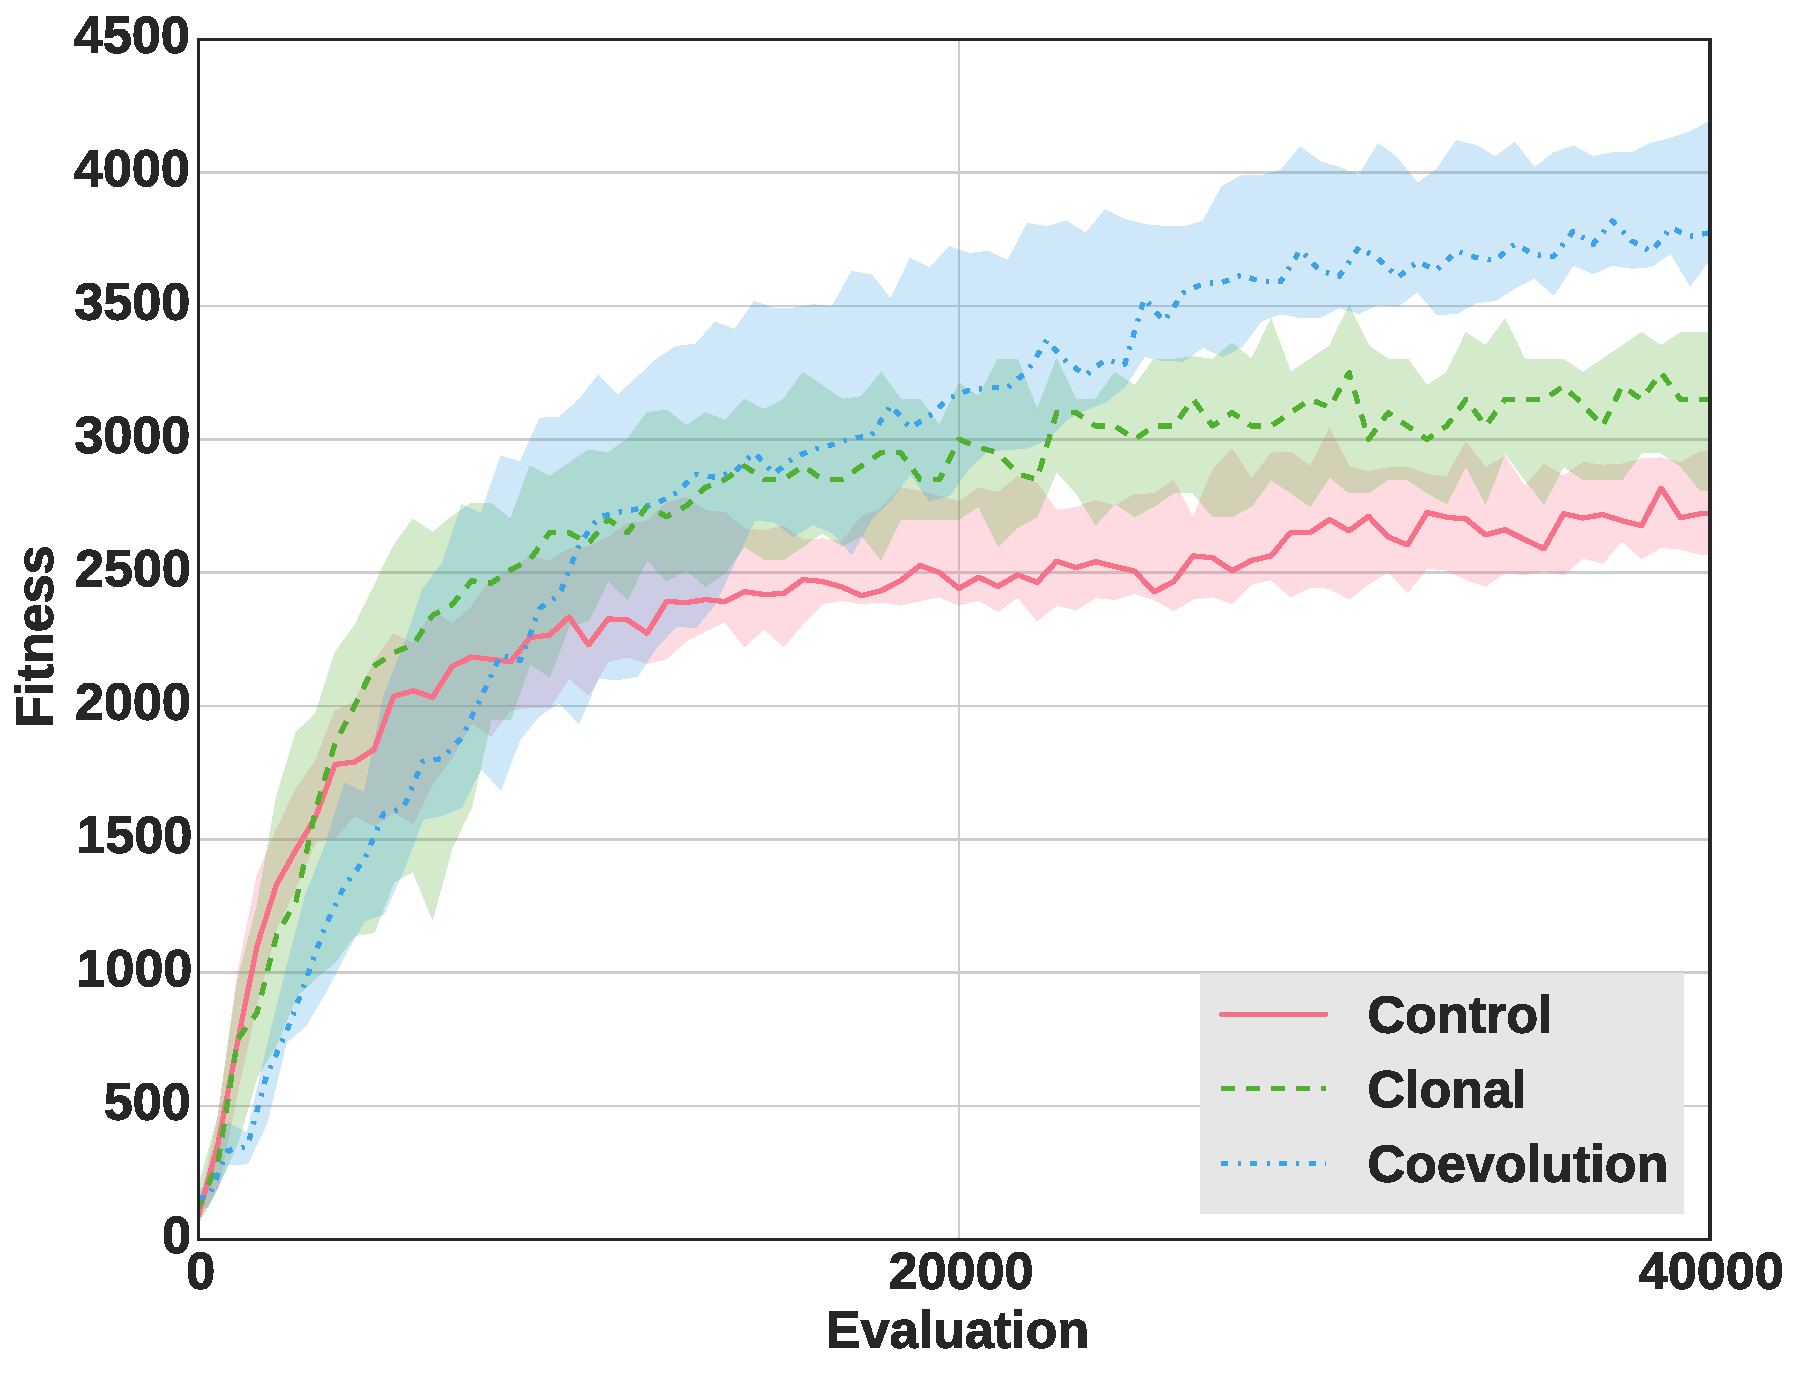
\includegraphics[scale = 0.40]{fig/ArticleRob1/fitnessHuntingStags.pdf}
        \caption{\textbf{Performance of the cooperative solutions.}
        Median fitness score of the best individuals in each of the runs where cooperation evolved for each setup over time. The fitness score of an individual is computed as the average reward the individual earned per trial by foraging targets. The colored areas around the medians represent the first and third quartiles.} 
        \label{fig:HuntingFitness}
      \end{center}
    \end{figure}

    However, cooperative individuals do not perform with the same \emph{efficiency} from one setup to another. We show in Figure~\ref{fig:HuntingFitness} the median fitness score of the best individuals in each independent run where cooperation evolved over time and for each setup. Fitness scores are significantly different in each setup with the best score obtained in the coevolution setup and the worst in the control setup (Mann-Whitney U-test on the fitness score of the best individuals at the last evaluation, {\em p}-value $< 0.001$).

    These differences in efficiency can be explained by looking at the nature of the cooperative behaviors evolved, which reveals two types of behaviors: \emph{turning} and \emph{leader/follower}.

    Individuals adopting the turning strategy turn around one another so that they always see the other individual as well as stay close to it (Figure~\ref{fig:behaviorTracesHunting}(A)). This allows the two individuals to approach simultaneously a same target and therefore forage it in a cooperative fashion. In this strategy, both individuals have a similar behavior and no role division is necessary for their successful cooperation.

    In comparison, individuals which evolve a leader/follower strategy adopt a differentiation between two roles: \emph{leader} and \emph{follower} (Figure~\ref{fig:behaviorTracesHunting}(B)). The individual we call leader always goes first on a target whereas the follower always arrives second on the same target. We observe that the follower's behavior consists in staying close to the leader and always keeping it in front of itself. In comparison the leader shows a lesser interest in the presence of its follower and rarely checks on its position.

    \begin{figure}[h]
      \centerfloat
        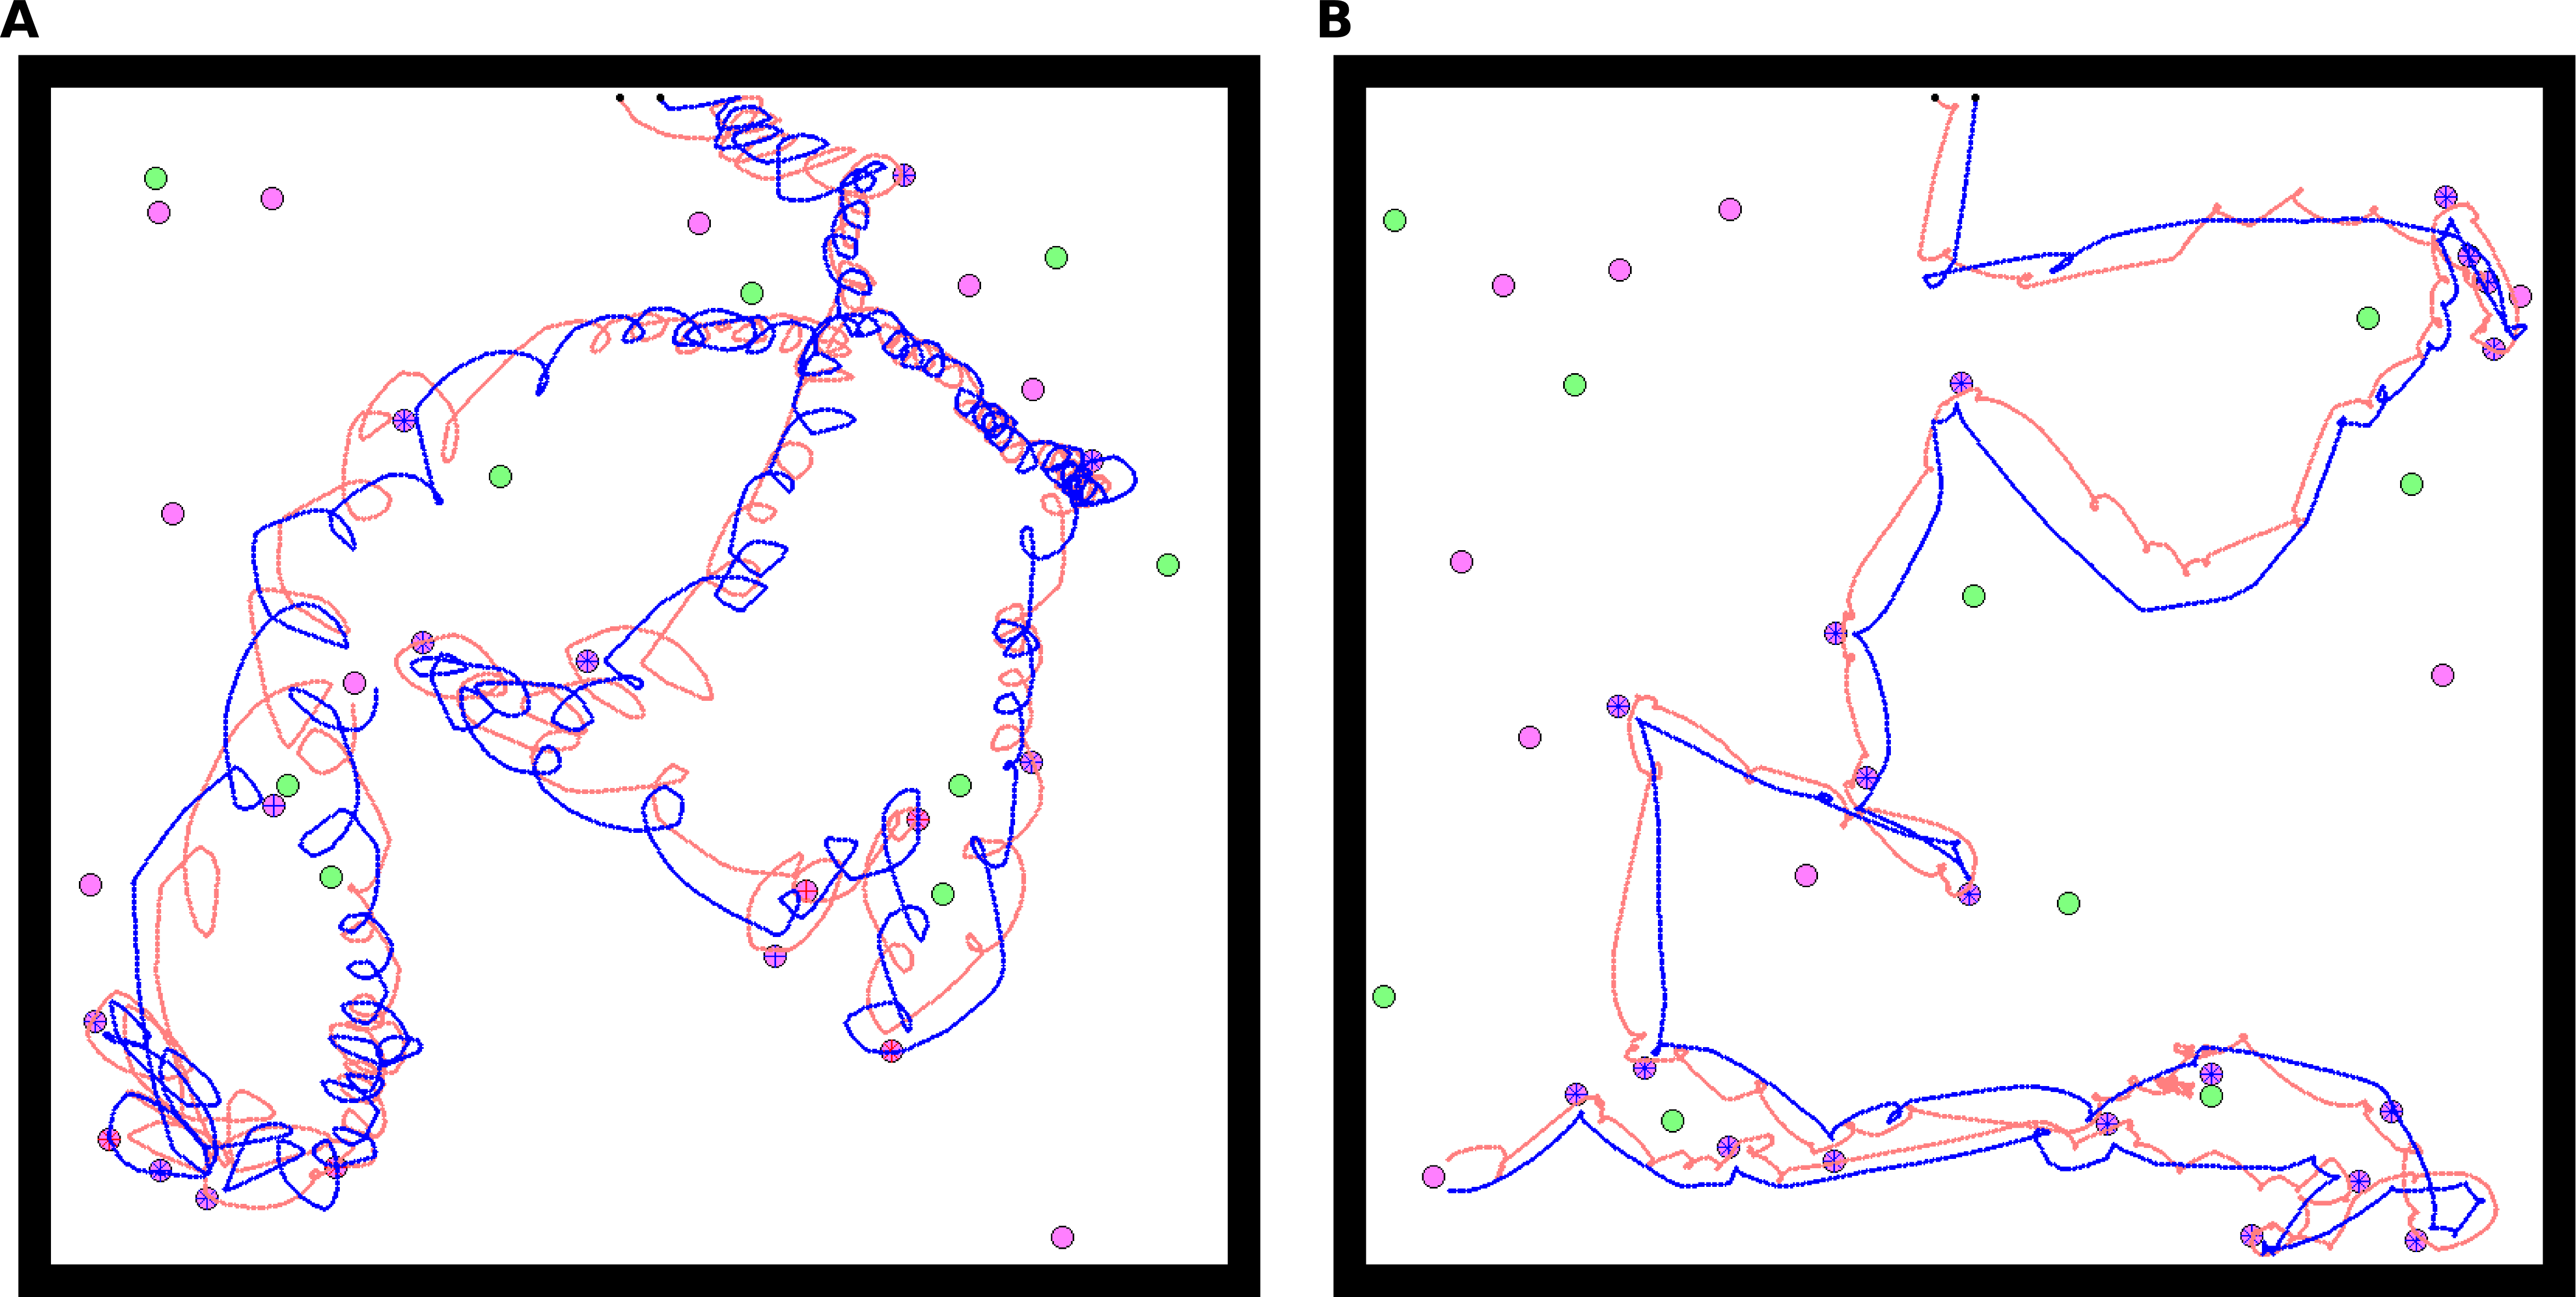
\includegraphics[scale=0.8]{fig/ArticleRob1/figBehaviours.png}
      \caption{\textbf{Snapshots of the simulation after an entire trial in the foraging task.}
      The path of each robotic agent from their initial positions (black dots) is represented in red and blue. The green and purple discs represent the 18 targets in the environment. When a target is foraged by the two agents, a red cross (resp. blue) is drawn on the target if the red agent (resp. blue) arrived on it first. Each snapshot corresponds to a trial where agents adopted a different behavior: {\em (A)}~turning or {\em (B)}~leader/follower.}
      \label{fig:behaviorTracesHunting}
    \end{figure}


    Table~\ref{tab:ForagingBehaviors} shows the distribution of cooperative strategies for all three setups. Whereas the control and clonal setups always resulted in turning strategies (resp. 10/10 and 28/28), the coevolution setup always displayed the evolution of a leader/follower strategy (14). We observe that this latter strategy leads to more efficient cooperation. Indeed, individuals adopting the turning strategy are forced to check constantly on the other individual's position. Consequently, they cannot be as fast as individuals with a leader/follower strategy where they move to the target in a straight line under the leader's direction. Moreover, due to the random proximity of the targets, the turning strategy is prone to errors. Namely, they often get to another target than that of their partner whenever two targets are too close to each other.

    A possible explanation as to why no leader/follower strategy could evolve in the control and clonal setups may be because of the need to differentiate between the two roles. Indeed, there needs to be the existence of an asymmetry between the two individuals for this phenomenon to appear. With coevolved populations, this asymmetry is deliberately created by the separation between the two populations. Indeed, we observe that one population exclusively contains leaders while the other exclusively contains followers. 

    The two other setups fail to evolve heterogeneous behaviors. In the control setup, this may be due to the evolutionary algorithm used, especially with elistism enforcing the homogenization of the population throughout the course of evolution (as hinted in the Methods Section). Then, the clonal setup introduces yet another challenge as switching to a particular role can only be done during evaluation as both individuals are by definition genetically similar.

    \begin{table}[h]
      \center{
        \begin{tabular}{|l|c|c|c|}
          \hline
          \textbf{Setting} & \textbf{\# Leader/Follower} & \textbf{\# Turning} & \textbf{Total}\\ 
           & \textbf{Strategy} & \textbf{Strategy} & \\ 
          \hline
          \hline
          \textbf{Control} & 0 & 10 & \textbf{10}\\
          \hline
          \textbf{Clonal} & 0 & 28 & \textbf{28}\\
          \hline
          \textbf{Coevolution} & 14 & 0 & \textbf{14}\\
          \hline
        \end{tabular}
      }
      \caption{\textbf{Evolution of a cooperative strategy.}
      Repartition of the different strategies evolved in each of the runs where cooperation evolved for each setup in the foraging task. We indicate in each cell the number of simulations where a particular strategy evolved.}
      \label{tab:ForagingBehaviors}
    \end{table}

\section{Going Beyond the Evolvability vs. Efficiency Tradeoff using Incremental Evolution}

  The previous section revealed a tradeoff between evolvability and efficiency. In the clonal setup, cooperation evolves more often than with other setups. However, the coevolution setup yields cooperative behaviors which are more efficient, with paired individuals displaying asymmetrical behaviors.

  In this section, we address the following question: is it possible to benefit from both evolvability \textit{and} efficiency with the clonal and/or the coevolution setups? In other words, we explore (1) whether the clonal setup can be used to evolve pairs with heterogeneous behaviors, and (2) whether the coevolution setup can be improved in terms of number of runs where cooperation evolved.

  In order to address this question, we use incremental evolution, a rather common method in evolutionary robotics for solving challenging problems~\parencite{Dorigo1994,Saksida1997,Bongard2008,Doncieux2013}. The main principle is to ease the learning of a complex task by splitting it into simpler sub-tasks~\parencite{Perkins1996}.

  In the following, we introce an additional task, the \textit{waypoints crossing} task, which requires the evolution of coordination behaviors, and is simpler to address than the preous task. Individuals evolved in this first task are then used as starting point for the original task described earlier, hoping that cooperative behavior will be \emph{recycled} from the first task to the second task.
  
  \subsection{Waypoints Crossing Task}  

    We consider a task where robotic agents have to cross randomly positioned waypoints. As such, these round waypoints do not act as obstacles and have a diameter of 30 units. As soon as an agent goes through a waypoint, it can not be seen by this agent anymore. All 18 waypoints have the same color and can be crossed in any order. The fitness score (\(F\)) of each individual is defined as the average longest sequence of waypoints shared by both agents per trial:

    \[
    F = \frac{1}{N*M} \sum_{i=1}^{N} \sum_{j=1}^{M} l_{max_{ij}}
    \]

    Where \(N\) is the number of individuals encountered ($5$ in the control and coevolution setups, $1$ in the clonal setup), \(M\) the number of trials ($5$) and \(l_{max_{ij}}\) the longest sequence of waypoints shared by both individuals at trial \(j\) with individual \(i\).

    This implies that the two individuals are rewarded when crossing waypoints in the same order as well as maximizing the number of waypoints crossed. Each evaluation lasted $10000$ simulation steps and $60$ independent runs were conducted for each experimental setup, each one lasting $40000$ evaluations.

    \begin{figure}[h]
      \begin{center}
        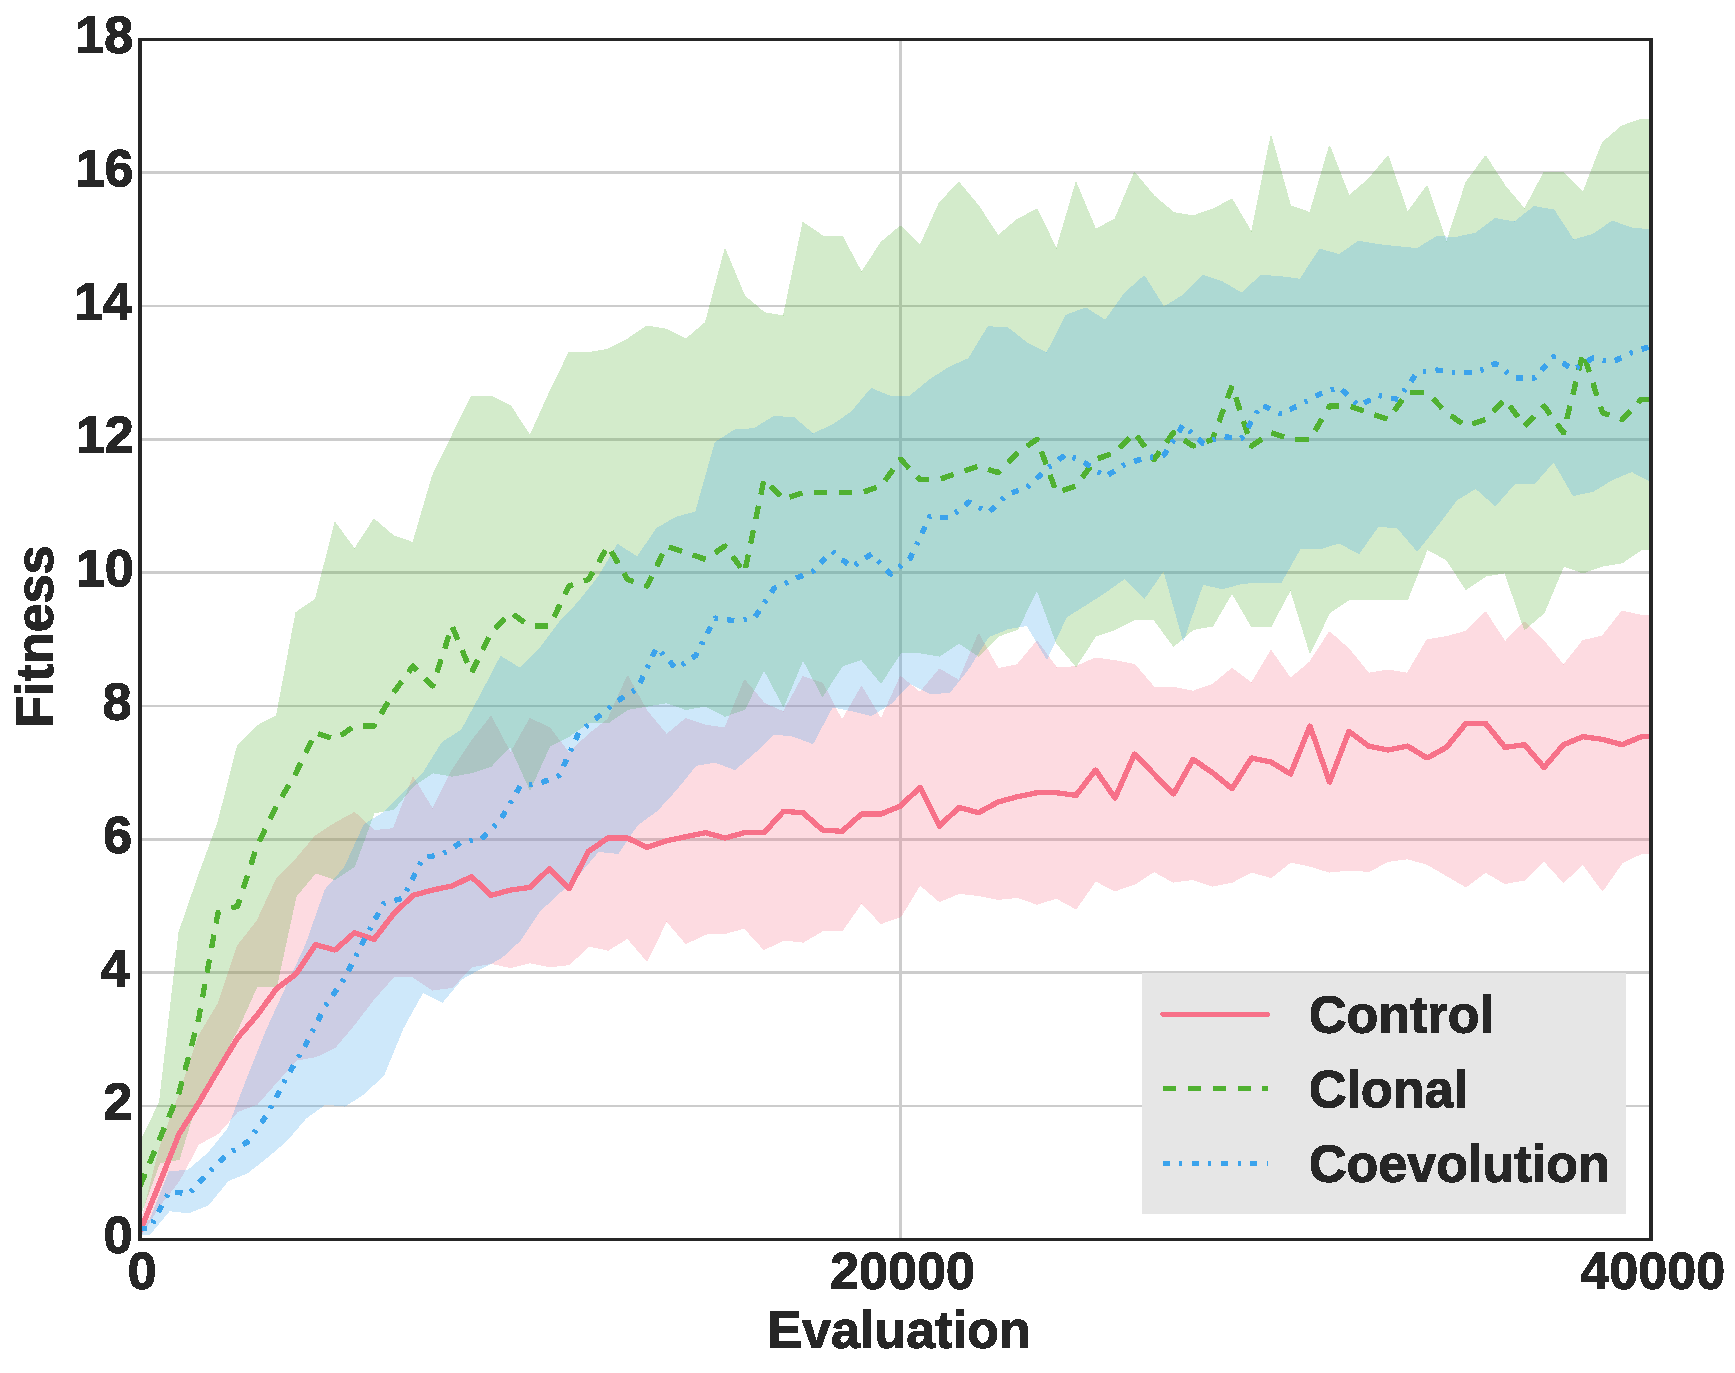
\includegraphics[scale = 0.4]{fig/ArticleRob1/fitnessWaypoints.pdf}
        \caption{\textbf{Performance of the cooperative solutions.}
        Median fitness score of the best individuals in each of the 60 independent runs and for each setup over time. Fitness score is computed as the average longest sequence of waypoints shared by both agents per trial. The colored areas around the medians represent the first and third quartiles.}
        \label{fig:WaypointsFitness}
      \end{center}
    \end{figure}

    All simulations showed an increase in fitness score for each of the three setups (cf. Figure~\ref{fig:WaypointsFitness}). This was expected as this task does not represent a particular challenge for the individuals: it simply needs the evolution of a successful coordination strategy. However, whereas the coevolution and clonal setups performed equally, they both surpassed the performance of individuals from the control setup (Mann-Whitney, {\em p}-value $< 0.001$).

    As with the previous foraging task, we can hypothesize that these differences in fitness scores are due to differences in the behaviors evolved. Table~\ref{tab:WaypointsBehaviors} gives a classification of the cooperative behaviors for each setup. They are similar to those in the previous task with the addition of a third rare strategy: the \emph{wall-following} strategy (which is regrouped in ``Other''). Wall-followers simply follow the walls around the arena and cross any waypoints close to the wall they are adjacent to. As such, this is a far less efficient strategy than the two others. 


    \begin{table}[h]
      \center{
        \begin{tabular}{|l|c|c|c|c|}
          \hline
          \textbf{Setting} & \textbf{\# Lead.} & \textbf{\# Turn.} & \textbf{\# Other} & \textbf{Total}\\ 
           % & \textbf{Strategy} & \textbf{Strategy} & \textbf{Strategy} & \\ 
          \hline
          \hline
          \textbf{Control} & 19 & 37 & 4 & \textbf{60}\\
          \hline
          \textbf{Clonal} & 23 & 31 & 6 & \textbf{60}\\
          \hline
          \textbf{Coevolution} & 59 & 1 & 0 & \textbf{60}\\
          \hline
        \end{tabular}
      }
      \caption{\textbf{Cooperative strategies evolved.}
      Repartition of the different strategies evolved in each of the 60 independent runs for each setup in the waypoints task. We indicate in each cell the number of simulations where a particular strategy evolved: \emph{Leader/follower} (Lead.), \emph{Turning} (Turn.) or \emph{Other}. ``Other'' regroups wall-following strategies or simulations where no recognizable strategy evolved.}
      \label{tab:WaypointsBehaviors}
    \end{table}

    \begin{figure}[h]
      \centerfloat
        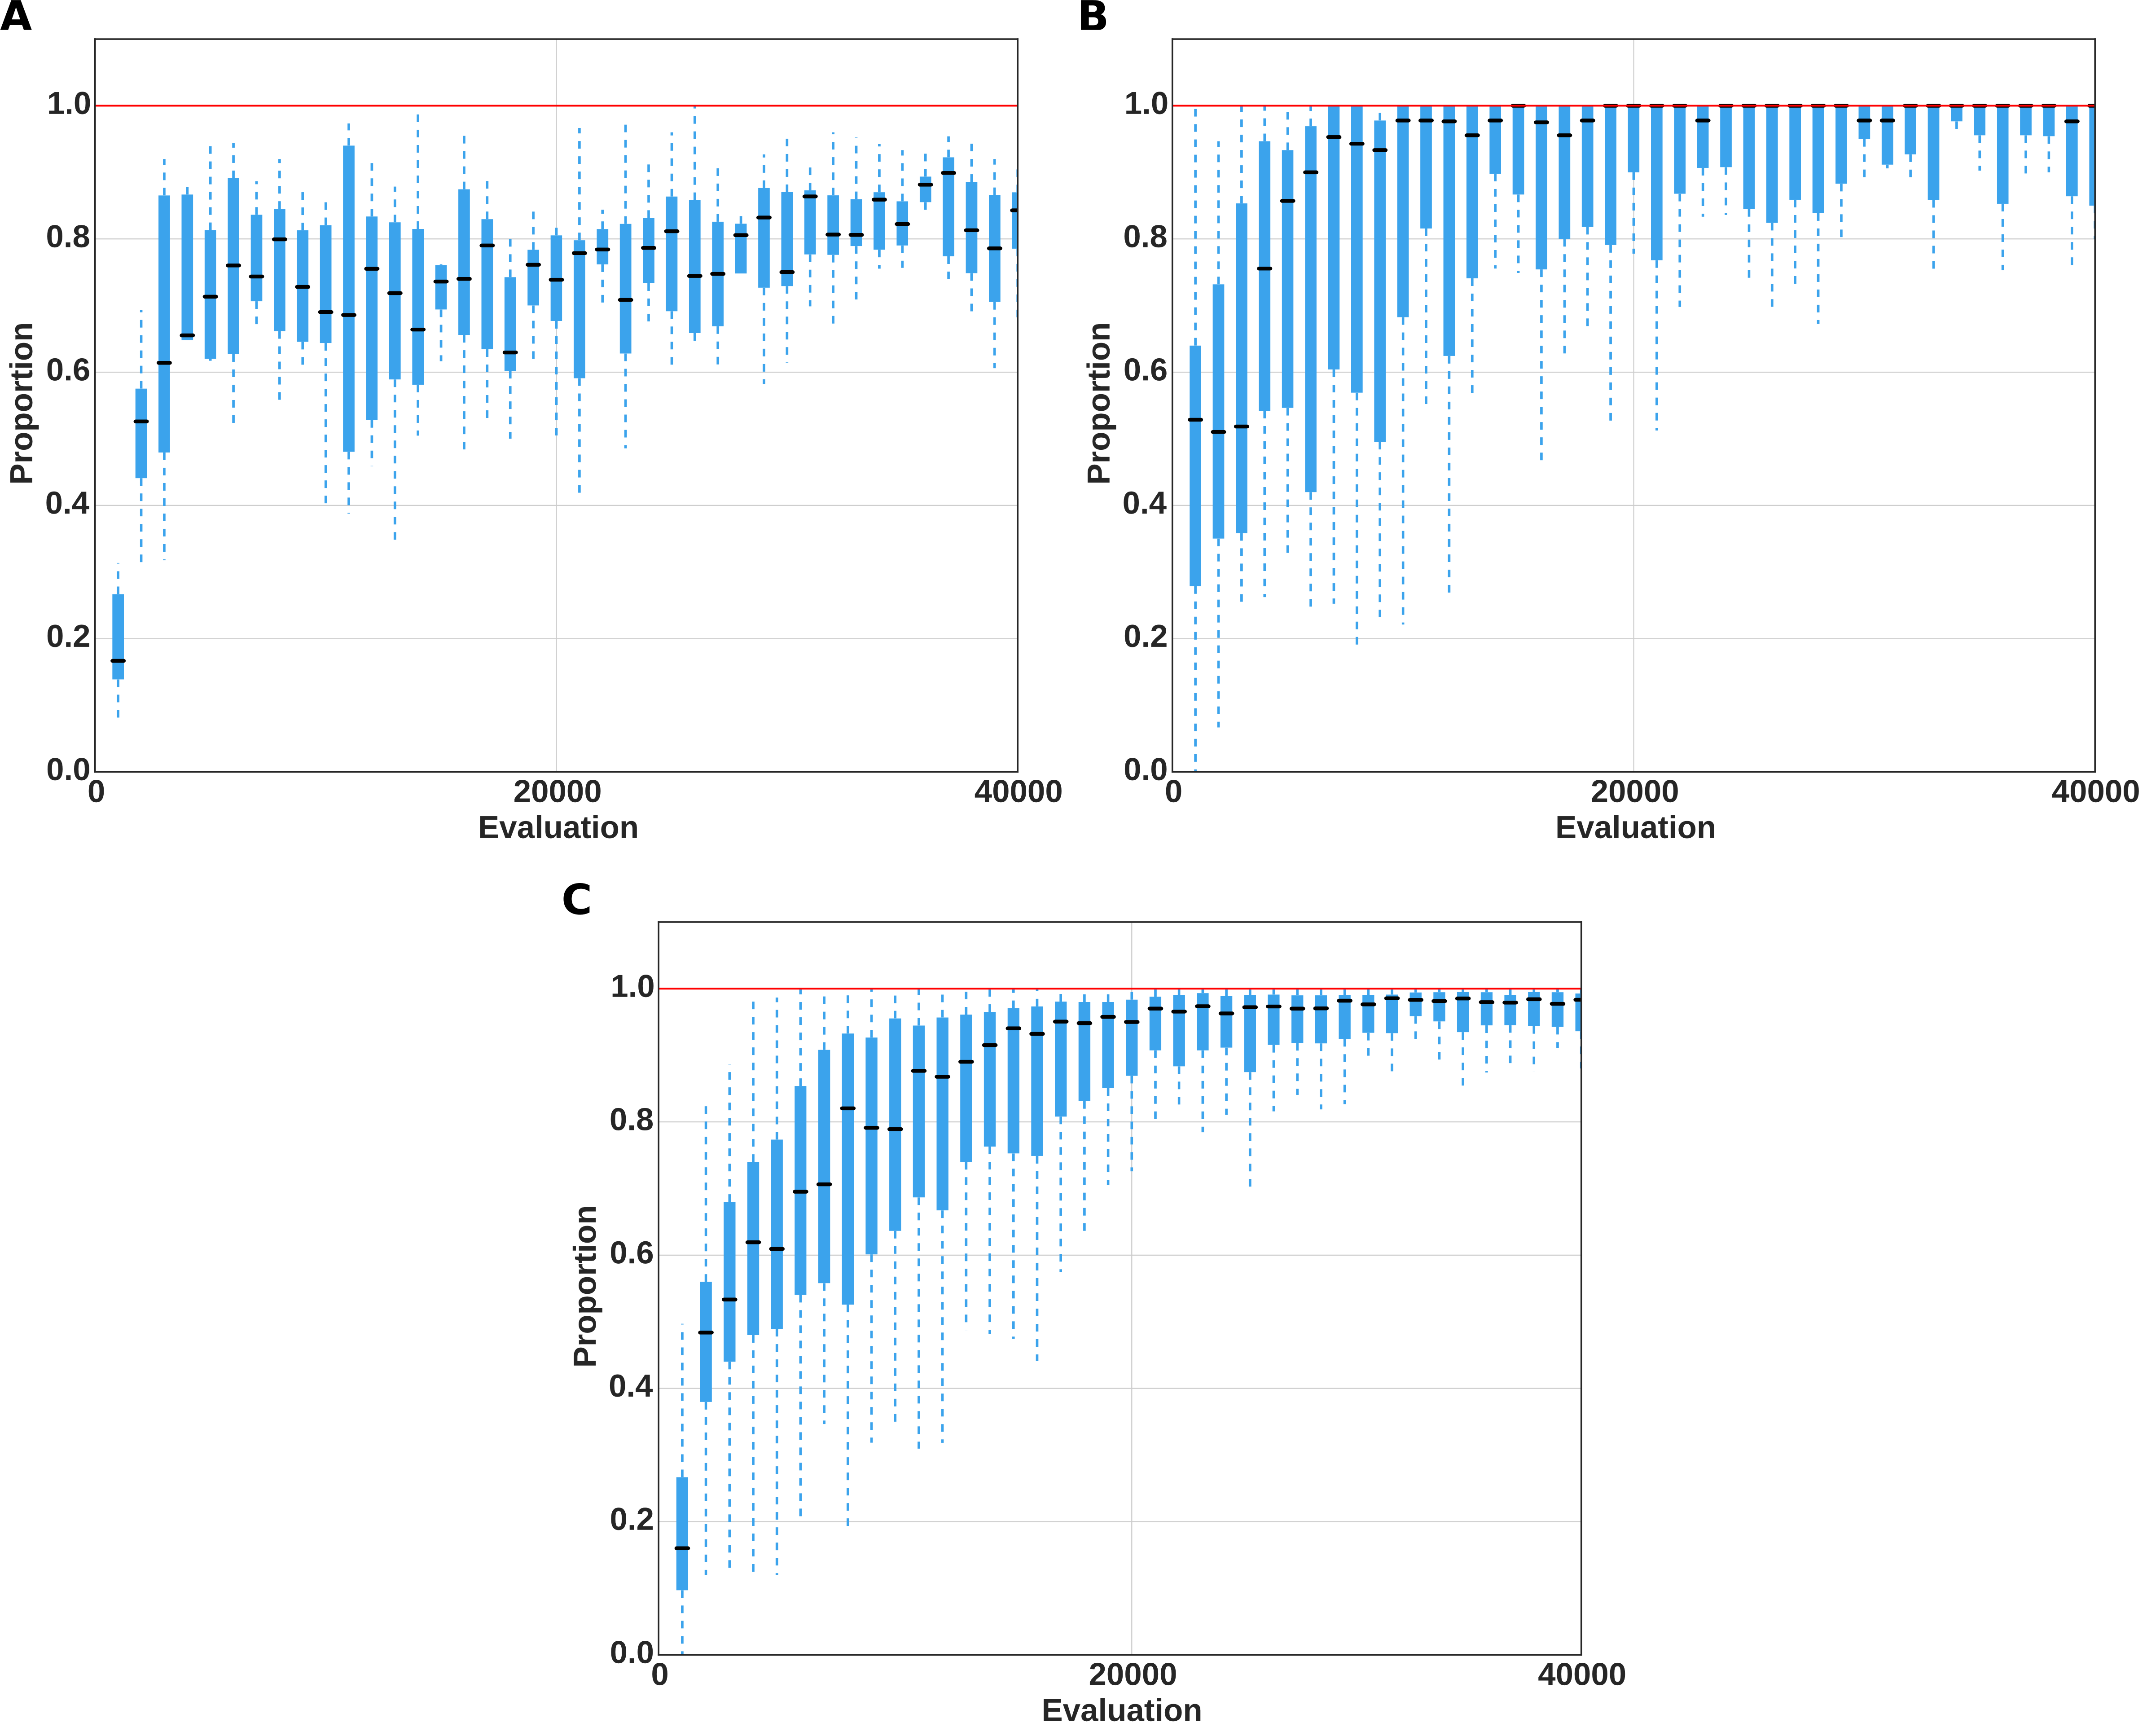
\includegraphics[scale=0.8]{fig/ArticleRob1/figLeadership.png}
      \caption{\textbf{Proportion of leadership.}
      Boxplots of the proportion of leadership over time for the best individuals in each runs where the proportion at the last evaluation was greater than 0.75 in the {\em (A)}~control, {\em (B)}~clonal or {\em (C)}~coevolution setup. This value represents the proportion of waypoints crossed by both individuals for which the leader arrived first.}
      \label{fig:WaypointsLeadership}
    \end{figure}

    In the coevolution setup, nearly all runs (59/60) evolved a leader/follower strategy. Interestingly, although fitness scores in the clonal and control setups are significantly different, this behavior evolved in roughly one third of the runs for both setups. To explain the difference in fitness scores, we must take into account the quality of the leader/follower strategy in each setup. We measure the proportion of leadership in each interaction, which is computed as the proportion of waypoints crossed by both individuals for which the leader arrived first. Figure~\ref{fig:WaypointsLeadership} displays the boxplots of the proportion of leadership for the best individuals in each setup and only for the simulations where a successful leader/follower strategy evolved (a minimal threshold of 0.75 is chosen to consider only the best performing runs). We show that the proportion of leadership is greater in the clonal and coevolution setups than in the control one (Mann-Whitney, {\em p}-value $< 0.005$). These differences means that the individuals are more efficient in their leader/follower strategy in the clonal and coevolution settings than in the control one. This explains the differences in fitness scores observed in Figure~\ref{fig:WaypointsFitness}.

    Interestingly, whereas in the foraging task no leader/follower strategy could evolve in the control and clonal setups, this strategy did evolve in one third of the simulations for this task. This could mean that these individuals use information in the environment to adopt one role or the other. Indeed, we observe that this is achieved by exploiting the differences in the initial starting positions, with one individual on the left and the other on the right. They both turn to the same direction (left or right, depending on the runs) at the beginning of the simulation which results in one individual (the leader) turning its back to the other, while the second individual (the follower) looking at its partner. 


  \subsection{Recycling Cooperative Behaviors in the Foraging Task}

    Coming back to the initial foraging task, we perform the exact same experiment described at the beginning of this Chapter, with one notable exception: the initial population is initialized with genomes evolved for solving the waypoint task. This implies that coordination is possible starting from the very first generation of each setup. Given that we have already shown that such coordination is a desirable feature, the question is: will it be possible to retain cooperative behaviors in order to solve the foraging task?

    \begin{table}[h]
      \center{
        \begin{tabular}{|l|c|c|c|c|}
          \hline
          \multirow{2}{*}{\textbf{Setting}} & \multicolumn{2}{c|}{\textbf{\# Coop.}} & \multirow{2}{*}{\textbf{\# Solitary}} & \multirow{2}{*}{\textbf{Total}}\\ 
          \cline{2-3}
           & \textbf{\# Lead.} & \textbf{\# Turn.} & & \\ 
          \hline
          \hline
          \textbf{Control} & 0 & 20 & 40 & \textbf{60}\\
          \hline
          \textbf{Clonal} & 0 & 24 & 36 & \textbf{60}\\
          \hline
          \textbf{Coevolution} & 28 & 0 & 32 & \textbf{60}\\
          \hline
        \end{tabular}
      }
      \caption{\textbf{Evolution of a cooperative strategy.}
      Proportion of the 60 independent simulations where the best individual evolved a cooperative strategy (collecting purple targets) or a solitary strategy (collecting green targets) for each setup in the foraging task when individuals are previously evolved in the waypoints task. In addition, the repartition of the different strategies is indicated when cooperation evolved: \emph{Leader/Follower} (Lead.) or \emph{Turning} (Turn.).}
      \label{tab:RecyclingCoopBehaviors}
    \end{table}

    Table~\ref{tab:RecyclingCoopBehaviors} gives the results in terms of evolved behaviors from the $60$ independent runs for each setup. 
    The coevolution setup evolves cooperation slightly more often (28/60) than both the control (20/60) and the clonal (24/60) setups. 
    A first remark is that the number of occurences of cooperation for the coevolution and control setups have actually doubled compared to previous results without incremental evolution (see Table~\ref{tab:ForagingCoop}). This is not the case for the clonal setup, which does not appear to benefit from incremental evolution. 

    A second remark is that cooperation in the coevolution setup systematically corresponds to a leader/follower strategy, which is \textit{never} the case with the two other setups. This has a significant, though expected, impact on fitness scores, as shown in Figure~\ref{fig:RecyclingFitness}. Cooperation evolved with the coevolution setup leads to significantly greater fitness scores (Mann-Whitney, {\em p}-value $<0.001$). 

    Results from this experiment make it possible to revise our initial statement. Using pre-trained individuals strongly benefits the coevolution setup in terms of evolvability. But this is not the case with the clonal setup, for which using pre-trained individuals improves neither evolvability nor efficiency. Therefore, we may face a tradeoff which does not concern evolvability and efficiency, but one that implies computational cost: the coevolution setup outperforms the clonal setup on both evolvability and efficiency \textit{at the cost of additional computational effort}.

    The control and clonal setups completely failed to maintain a leader/follower strategy, even though such strategy originally evolved. An explanation is provided by considering the difference between the waypoints task, where leader/follower evolved, and the current foraging task. In the waypoints task, symmetry breaking could be achieved at the beginning of the evaluation (as explained earlier), and could be retained afterwards as the follower was always behind the leader. However, the current foraging setup requires that the two robots display the same behavior to cooperatively collect a target (ie. both robots have to touch the target), which implies that leader/follower roles are lost, as they depend on the relative position of robots with one another. 


    \begin{figure}[h]
      \begin{center}
        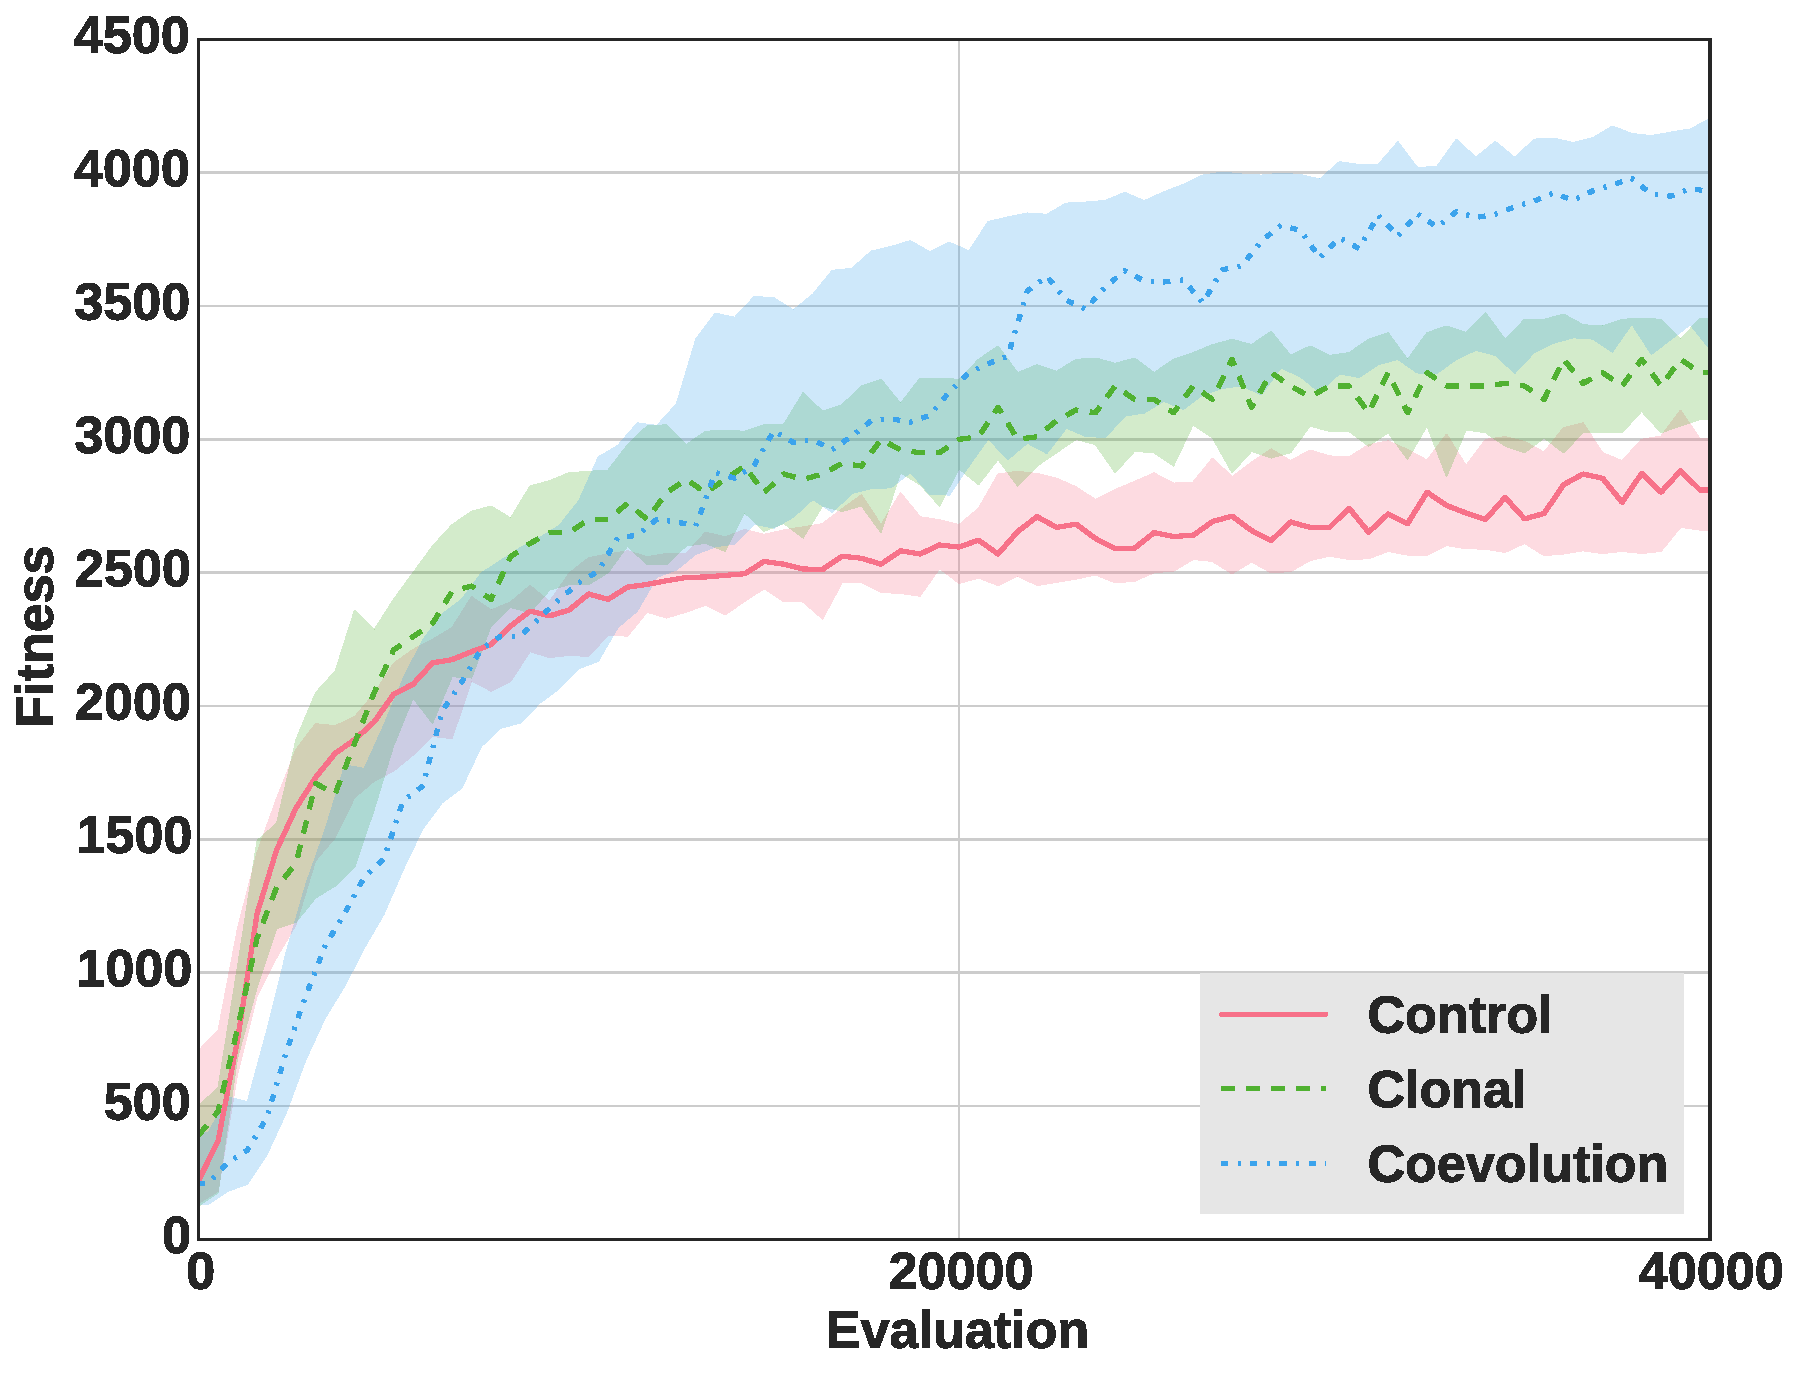
\includegraphics[scale = 0.4]{fig/ArticleRob1/fitnessRecyclingStags.pdf}
        \caption{\textbf{Performance of the cooperative solutions.}
        Median fitness score of the best individuals in each of the runs where cooperation evolved for each setup over time. The fitness score of an individual is computed as the average reward the individual earned per trial by foraging targets. The colored areas around the medians represent the first and third quartiles.}
        \label{fig:RecyclingFitness}
        \end{center}
    \end{figure}

\section{Discussion and Conclusion}

  In this Chapter, we considered several approaches for the evolution of cooperation in evolutionary robotics: a clonal approach, where all individuals in a group share the same genome, and a non-clonal approach, where individuals are independent from one another, but may share a common interest in cooperating. 

  We first showed that there exists a tradeoff between evolvability and efficiency. On the one hand, the clonal approach evolves cooperative behaviors on a more frequent basis than with the other approach. On the other hand, the non-clonal approach, which is implemented using a coevolution setup, results in more efficient behaviors in terms of pure performance whenever cooperation evolved. The non-clonal approach actually enables the evolution of asymmetric behaviors, such as a leader/follower strategy.

  We then used incremental evolution to evolve coordination behaviors using a simpler task in order to overcome this tradeoff and improve both evolvability and efficiency in each setup. We showed that while no improvement was observed in the clonal setup on either criteria, the outcome is very different for the coevolution setup: the probability of evolving cooperation actually increases, and the evolved cooperative solutions remain the most efficient.
 
  This work raises several questions. Firstly, heterogeneous behaviors were obtained with coevolution, a rather radical way to enable asymmetrical behaviors during cooperation. However, the waypoints task revealed that breaking symmetry can also be done with identical individuals using environmental feedback, even though such cooperation is difficult to obtain. As a consequence,  the evolution of cooperation with heterogeneous behavior without resorting to coevolution could be investigated. In particular, we could study how more elaborated neural architectures (e.g. using plasticity) can switch to a particular persistant regime depending on environmental cues available at the beginning of the evaluation.

  Secondly, incremental evolution requires an added computational cost in order to increase evolvability in the non-clonal approach. However, it may be possible to avoid this extra cost by considering other evolutionary methods. In particular, a multiobjective approach which considers both performance and \emph{diversity} could improve the optimization process~\parencite{Lehman2008, Doncieux2014a}. Though this approach looks promising, it is not clear yet how diversity should be implemented in the context of cooperative problem solving.